\documentclass[10pt,twocolumn,letterpaper]{article}

\usepackage[table]
\usepackage{cvpr}
\usepackage{times}
\usepackage{epsfig}
\usepackage{graphicx}
\usepackage{caption}
\usepackage{subcaption}
\usepackage{amsmath}
\usepackage{amssymb}
\usepackage{cite}

\usepackage{hhline}
\usepackage{pgf}
\usepackage{float}

% Include other packages here, before hyperref.

% If you comment hyperref and then uncomment it, you should delete
% egpaper.aux before re-running latex.  (Or just hit 'q' on the first latex
% run, let it finish, and you should be clear).
%\usepackage[pagebackref=true,breaklinks=true,letterpaper=true,colorlinks,bookmarks=false]{hyperref}

\cvprfinalcopy % *** Uncomment this line for the final submission

\def\cvprPaperID{****} % *** Enter the CVPR Paper ID here
\def\httilde{\mbox{\tt\raisebox{-.5ex}{\symbol{126}}}}

% Pages are numbered in submission mode, and unnumbered in camera-ready
%\ifcvprfinal\pagestyle{empty}\fi
\setcounter{page}{1}
\begin{document}

%%%%%%%%% TITLE
\title{Autonomously Classifying Facial Attractiveness}

%\author{Steven Hickson, Andrew Vaziri, Matthew O'Brien \\
%Georgia Institute of Technology\\
%{\tt\small me@stevenhickson.com, avazari3@gatech.edu, mjobrien@gatech.edu}
%}
\author{Team 4}

\maketitle
%\thispagestyle{empty}


%%%%%%%%% BODY TEXT
\section{Introduction}
With online dating continuing to grow, there is a natural
demand to make automatic recommendations. While
beauty isn’t objective, the preferences of a single person
may be. A system that could accurately rank other participants,
in terms of a target users inclination or in terms of a large general agreement, would have
great practical benefit in the world of social networks and online dating.
Beyond application, modeling individual’s attractions
may provide insight in the field of psychology. Physical
attraction is well established as a major component of forming
relationships. Tools to predict attraction between anonymous
participants could improve experimental studies. On
the theoretical side, component analysis may lead to new
insights about what features are universally attractive, and
what features are more personalized. We propose a method that 
autonomously rates a face's attractiveness based on the PCA decomposition of the image.
 
\section{Related Work}
Surveying the literature, there has been little work on
creating a mathematically rigorous human facial attractiveness
prediction other than \cite{eisenthal2006facial, kagian2006humanlike, kagian2008machine}, which all focus on a
machine learning approach using custom feature vectors
the authors have constructed by annotating key points on
the image and calculating measures such as the width and
height of various facial features as well as their relative proportions.
However, this approach is time-consuming and
not autonomous. Furthermore, subtle errors are induced by
noise in the annotation points, and some of the features used
are poorly defined. For example, one feature from [2] is to
have an operator choose a ”window representative of skin
smoothness” from the face. These approaches are also limited
in that they only classify attractiveness as a Boolean
function: attractive or unattractive. This and their 
lack of annotated data prevent them from using a purely autonomous model.

\section{Approach}
The first challenge in creating a suitable method is to obtain a good data set. To be suitable for machine learning the data set should be sufficiently large such that many attractive and unattractive examples are available. Furthermore, the set should be labeled with attractiveness scores that are based on face information only. In practice it is very difficult to find such a data set because people tend to skew towards higher ratings, and most public attractiveness rating websites include photographs with multiple people, full body photography, facial fashion accessories, a variety of facial expressions and other extraneous information such as background location. Once these challenges can be overcome there is the additional challenge of normalizing and registering the images to prepare them for feature extraction. Ideally all images should be the same size, have the eyes and mouths aligned, use a consistent background, constant lighting conditions and be capturing a face in full face view, meaning from directly in front. We collected images from a variety of sources and found that no data set met all these requirements. In the end we prioritized having a large data set of 2253 images, obtained from \cite{dataset}, all of which were rated on the site \emphasis{hotornot.com} and registered from a full face or nearly full face perspective using the technique described in \cite{berg2004names}. This data set was sub-optimal in that it included a variety of facial expressions and the ratings were done on the full photographs, not the cropped and registered images. However, it is the best and largest available. It should also be noted that this data set includes only female faces, just as in \cite{eisenthal2006facial, kagian2006humanlike, kagian2008machine}.

For feature vector construction, PCA decomposition was used to extract eigenfaces. Eigenface decomposition treats every image as a vector, and first calculates a mean image from the entire set of images. Then, principle component analysis is performed over the difference between each image and the mean image. This returns a set of basis vectors, called eigenfaces, that are linearly uncorrelated. The images of the eigenfaces most correlated with attractiveness can be seen in figure~\ref{fig:corfaces}. The first few eigenfaces will hold the most information and will together form a blurry image of a face. Later eigenfaces hold more detailed high frequency information.

This process returns N eigen faces where N is the number of face images in the data set. Any face image can be reconstructed by taking a weighted sum of the eigenfaces, with the weights being the eigenvalues associated with a particular person's face. The vector of N eigenvalues is the feature vector which we fed into our machine learning algorithm. 

\begin {figure} [h]
    \centering
        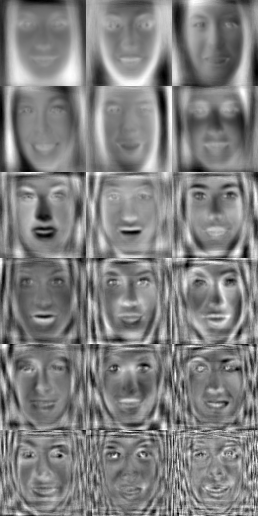
\includegraphics[width = \linewidth]{eigens.png}
    \label{fig:corfaces}
    \caption{The top correlated eigenfaces, in order of strongest to weakest}
\end {figure}

 With feature vectors for the rated images, techniques from machine learning could be applied to look for correlations and 
 to try and predict scores of new images. K Nearest Neighbors (KNN) is a technique that finds the K closest training examples in a feature space. The classification of the new test example is the class with the most neighbors. For our final implementation, images were divided into four bins, or classes, based on their score. New images looked at the four closest neighbors. Given a tie, the algorithm defaulted to the lower ranked class. The training data contained more attractive faces, and thus KNN was biased somewhat to claim images were more attractive. More details on this are presented in discussion.

\section{Evaluation}

Ninety percent of the images were separated for training, and the final ten percent saved for testing. Figure~\ref{table:conf_knn} displays the results of s

\begin{table}[h!]
\begin{center}
\noindent\begin{tabular}{c|c|c|c|c}
 \multicolumn{3}{c}{K Nearest Neighbors}  \\ \hhline{~*4{|-}|}
 \multicolumn{1}{c}{0} & 
 \multicolumn{1}{c}{1} & 
 \multicolumn{1}{c}{2} &
 \multicolumn{1}{c}{3} \\ \hhline{~*4{|-}|}
 0 & 2 & 1 & 5 & 2 \\ \hhline{~*4{|-}|}
 1 & 4 & 10 & 17 & 13 \\ \hhline{~*4{|-}|}
 2 & 1 & 11 & 34 & 34 \\ \hhline{~*4{|-}|}
 3 & 0 & 8 & 37 & 47 \\ \hhline{~*4{|-}|}
 \\
 \multicolumn{3}{c}{Closest eigenvalue L2 Norm match}  \\ \hhline{~*4{|-}|}
 \multicolumn{1}{c}{0} & 
 \multicolumn{1}{c}{1} & 
 \multicolumn{1}{c}{2} &
 \multicolumn{1}{c}{3} \\ \hhline{~*4{|-}|}
 0 & 2 & 0 & 5 & 3 \\ \hhline{~*4{|-}|}
 1 & 0 & 14 & 15 & 15 \\ \hhline{~*4{|-}|}
 2 & 4 & 8 & 31 & 37 \\ \hhline{~*4{|-}|}
 3 & 1 & 16 & 36 & 39 \\ \hhline{~*4{|-}|}
 \\
 \multicolumn{3}{c}{L2 Norm of Means of correlated eigenvalues}  \\ \hhline{~*4{|-}|}
 \multicolumn{1}{c}{0} & 
 \multicolumn{1}{c}{1} & 
 \multicolumn{1}{c}{2} &
 \multicolumn{1}{c}{3} \\ \hhline{~*4{|-}|}
 0 & 7 & 2 & 1 & 0 \\ \hhline{~*4{|-}|}
 1 & 16 & 9 & 19 & 0 \\ \hhline{~*4{|-}|}
 2 & 21 & 16 & 43 & 0 \\ \hhline{~*4{|-}|}
 3 & 25 & 11 & 56 & 0 \\ \hhline{~*4{|-}|}
 \\
 \multicolumn{3}{c}{Mean of L2 Norms of correlated eigenvalues}  \\ \hhline{~*4{|-}|}
 \multicolumn{1}{c}{0} & 
 \multicolumn{1}{c}{1} & 
 \multicolumn{1}{c}{2} &
 \multicolumn{1}{c}{3} \\ \hhline{~*4{|-}|}
 0 & 7 & 2 & 0 & 1 \\ \hhline{~*4{|-}|}
 1 & 21 & 6 & 0 & 17 \\ \hhline{~*4{|-}|}
 2 & 26 & 11 & 0 & 43 \\ \hhline{~*4{|-}|}
 3 & 33 & 7 & 0 & 52 \\ \hhline{~*4{|-}|}
 \\
 \multicolumn{3}{c}{SVM of eigenvalues}  \\ \hhline{~*4{|-}|}
 \multicolumn{1}{c}{0} & 
 \multicolumn{1}{c}{1} & 
 \multicolumn{1}{c}{2} &
 \multicolumn{1}{c}{3} \\ \hhline{~*4{|-}|}
 0 & 0 & 10 & 0 & 0 \\ \hhline{~*4{|-}|}
 1 & 0 & 44 & 0 & 0 \\ \hhline{~*4{|-}|}
 2 & 0 & 80 & 0 & 0 \\ \hhline{~*4{|-}|}
 3 & 0 & 92 & 0 & 0 \\ \hhline{~*4{|-}|}
 \\
 \multicolumn{3}{c}{Council of Experts}  \\ \hhline{~*4{|-}|}
 \multicolumn{1}{c}{0} & 
 \multicolumn{1}{c}{1} & 
 \multicolumn{1}{c}{2} &
 \multicolumn{1}{c}{3} \\ \hhline{~*4{|-}|}
 0 & 5 & 1 & 2 & 2 \\ \hhline{~*4{|-}|}
 1 & 8 & 5 & 9 & 22 \\ \hhline{~*4{|-}|}
 2 & 11 & 9 & 17 & 43 \\ \hhline{~*4{|-}|}
 3 & 9 & 7 & 20 & 56 \\ \hhline{~*4{|-}|}
 \\
 \multicolumn{3}{c}{Human Test}  \\ \hhline{~*4{|-}|}
 \multicolumn{1}{c}{0} & 
 \multicolumn{1}{c}{1} & 
 \multicolumn{1}{c}{2} &
 \multicolumn{1}{c}{3} \\ \hhline{~*4{|-}|}
 0 & 5 & 5 & 0 & 0 \\ \hhline{~*4{|-}|}
 1 & 9 & 22 & 11 & 2 \\ \hhline{~*4{|-}|}
 2 & 2 & 27 & 39 & 12 \\ \hhline{~*4{|-}|}
 3 & 0 & 11 & 42 & 39 \\ \hhline{~*4{|-}|}
\end{tabular}\par\bigskip
\caption{\small Confusion matrices}
\label{table:conf_knn}
\end{center}
\end{table}

\section{Discussion}

One major challenge for this project was volume of data. Though over 2200 images is a good start, there is still a lot of variety between images based on facial expression, lighting, and image perspective. Given all of these features, an image may have a much smaller subset of similar training examples to base its classification on. This was especially true for the lower scoring classes. There seems to be a natural bias towards more attractive images, and it caused our classification of the lower bins less accurate. Specifically, KNN will naturally bias towards the classes with more examples. However, reducing all training example to the number for our lowest class left far too little data. Some basic weighting schemes were tried to offset this trend, however none improved our final results.

Correlations between specific eigenvectors and the attractiveness scores were examined. Neither principle component anaylsis nor direct correlation showed any significant trends, and only using the most correlated vectors did not improve any of our results. This could mean individual eigenvectors do not correlate to attractiveness well, or that our data set was simply too small. Observing figure ~\ref{fig:mean_faces}, one can easily see a trend between classes, especially related to the shape of the face outline. Referring to figure ~\ref{fig:corfaces} again, one can see the top two correlated eigenvectors represent this feature. These results seem to indicate the eigenvectors are representing at least some features directly correlated to attraction.

\begin {figure} [h]
    \centering
    \begin {minipage}{0.22\textwidth}
        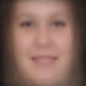
\includegraphics[width = \linewidth]{mean_0.png}
    \end {minipage}
    \begin {minipage}{0.22\textwidth}
        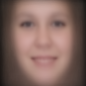
\includegraphics[width = \linewidth]{mean_1.png}
    \end{minipage}
    \begin {minipage}{0.22\textwidth}
        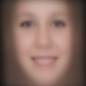
\includegraphics[width = \linewidth]{mean_2.png}
    \end {minipage}
    \begin {minipage}{0.22\textwidth}
        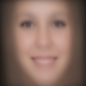
\includegraphics[width = \linewidth]{mean_3.png}
    \end{minipage}
    \label{fig:mean_faces}
    \caption{The mean faces for each class}
\end {figure}

-->Why did we reject SVM?
-->How did we use decision trees?

\cite{turk1991eigenfaces, belhumeur1997eigenfaces, yang2002kernel, guo2000face, eisenthal2006facial, }

%-------------------------------------------------------------------------

{\small
\bibliographystyle{ieee}
\bibliography{egbib}
}

\end{document}
